\section{Utilisation du logiciel}

Les deux objectifs présentés en \ref{obj} étaient à l'origine plus vagues. Nous avions le choix entre pousser l'analyse très loin et ne pas faire une interface graphique très évoluée, ou trouver un juste milieu. Ambitieux, nous souhaitions pousser l'analyse loin et réaliser une interface graphique évoluée.

\subsection{Fonctionnement global}
A partir de fichiers de données recensant la topologie d'internet et sa structure. Nous devons, en outre, construire un graphe et permettre son affichage dans une fenêtre en Qt.

Nous venons de voir que la base de l'application est \textit{Boost} et que nous avons adopté le pattern MVC afin de développer de manière plus sereine. La coeur de ce système est la communication entre le modèle et la vue, en d'autres termes : le contrôleur. Voyons ce qu'il permet de faire :
\begin{itemize}
 \item Lancer la lecture des fichiers de données afin de construire le graphe,
\item obtenir le nombre d'AS, de liens, et d'autres informations globales sur le graphe,
\item de récupérer le graphe sans les stubs,
\item de récupérer l'adjacence d'un AS,
\item de récupérer les informations concernant un AS (centrality, numéro),
\item de ne récupérer qu'une partie du graphe en fonction de la centralité des sommets,
\item de calculer les coordonnées que les sommets doivent avoir sur l'interface graphique.
\end{itemize}






ATTENTION : \'ebauche pour cette partie.
\subsection{Description du programme}

Le programme tel que le voit l'utilisateur est une fen\^etre graphique avec un menu en haut, une zone d'affichage au centre, et une zone de notification en bas.

\begin{figure}[ht]
\centering
 \fbox
 {
 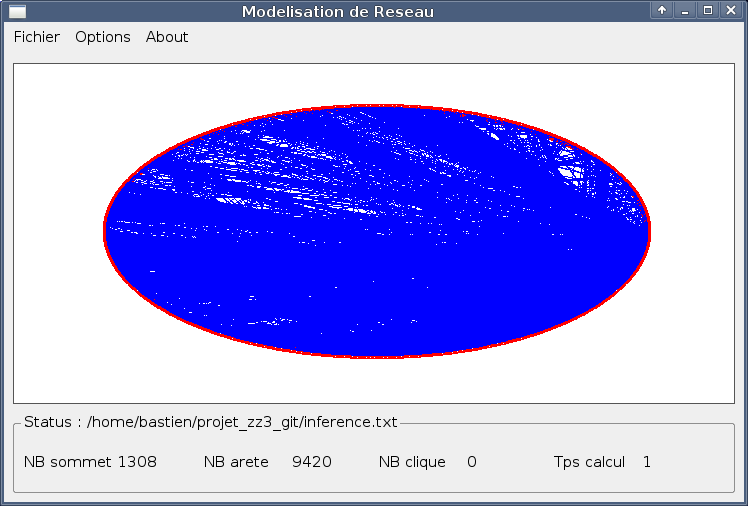
\includegraphics[width=16cm]{./schema/capture_ecran_programme.png}
 }
  \caption{\label{ecran_principal}Ecran principal du programme}
\end{figure}


Le menu comporte trois types d'entr\'ees :
\begin{description}
 \item[Fichier] permet l'ouverture des fichiers de donn\'ees \`a lire ou la fermeture du programme,
 \item[Options] permet les interactions avec le graphe telles que l'effacement de la zone d'affichage ou encore les recherche d'informations sur un AS,
 \item[About] permet l'affichage d'informations sur le programme.
\end{description}

\subsection{L'exp\'erience utilisateur}
\par
Lors du lancement du programme, l'utilisateur se retrouve devant un fen\^etre o\`u la zone d'affichage est vide et les compteurs de la zone de notification sontt tous \`a z\'ero comme c'est le cas sur la figure \ref{ecran_principal}.
\par
\`A ce stade l\`a, l'utilisation des options ne lui est d'aucune utilit\'e. Il peut aller dans le menu \textit{About} pour avoir des informations sur le programme, comme montrt\'e figure \ref{ecran_about}.

\begin{figure}[ht]
\centering
 \fbox
 {
 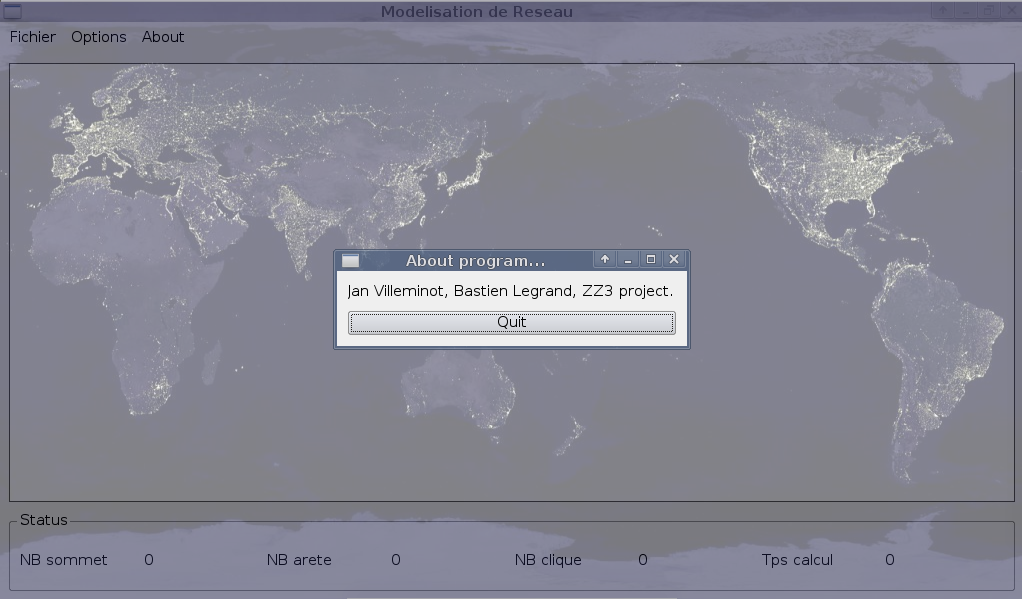
\includegraphics[width=16cm]{./schema/capture_ecran_about.png}
 }
  \caption{\label{ecran_about}Informations sur le programme}
\end{figure}

\par
Il peut aussi d\'ecider d'aller explorer le menu \textit{Fichier}, ce qui lui laissera le choix entre ouvrir un fichier de donn\'ees pour construire un graphe ou quitter le programme. Ce menu est illustr\'e figure \ref{ecran_fichier}.

\begin{figure}[ht]
\centering
 \fbox
 {
 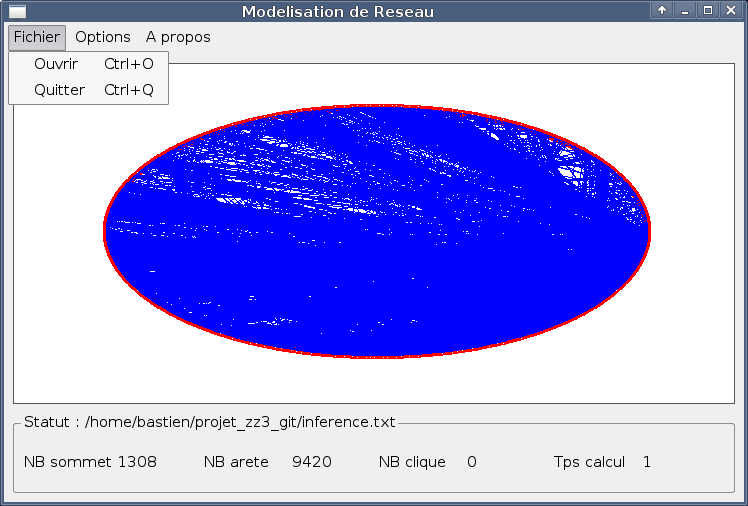
\includegraphics[width=16cm]{./schema/capture_ecran_fichier.png}
 }
  \caption{\label{ecran_fichier}Ecran principal du programme}
\end{figure}

S'il choisit d'ouvrir un fichier de donn\'ees, une nouvelle fen\^etre de navigation s'ouvre et lui demande de choisir son fichier, c'est la figure \ref{ecran_donnees}

\begin{figure}[ht]
\centering
 \fbox
 {
 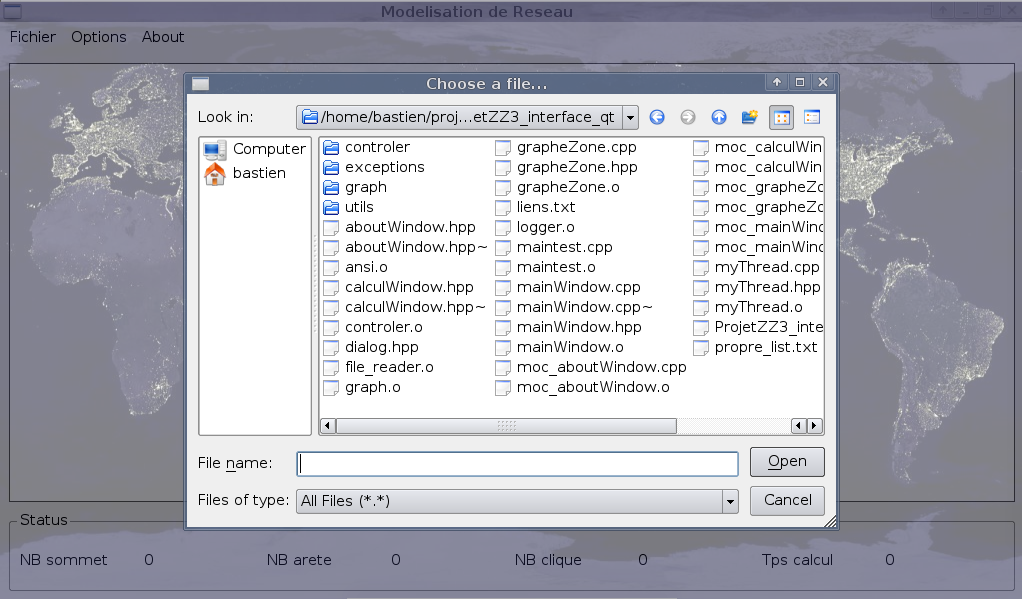
\includegraphics[width=16cm]{./schema/capture_ecran_donnees.png}
 }
  \caption{\label{ecran_donnees}Ecran principal du programme}
\end{figure}

L'utilisateur choisit un fichier de donn\'ees \`a ouvrir et le logiciel se charge d'afficher le graphe correspondant en organisant les sommets sur un polyg\^one r\'egulier \`a n c\^ot\'es.
La barre de status est mise \`a jour avec des informations telles que le nombre de sommets, le nombre d'ar\^etes ou le nombre de clique. Il obtient ainsi un \'ecran comme on peut en voir un figure \ref{ecran_graph}

\begin{figure}[ht]
\centering
 \fbox
 {
 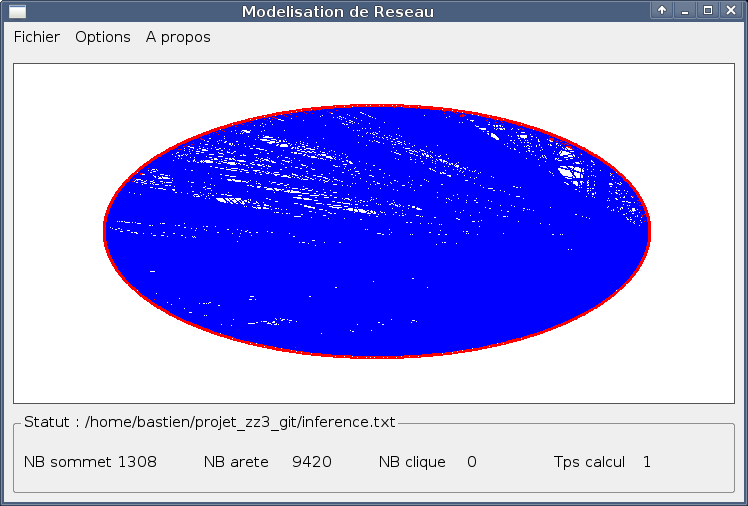
\includegraphics[width=16cm]{./schema/capture_ecran_graph.png}
 }
  \caption{\label{ecran_graph}Ecran principal du programme}
\end{figure}